\documentclass[pra,12pt]{revtex4}
\usepackage{amsmath}
\usepackage{amssymb}
\usepackage{graphicx}
\usepackage{color}
\usepackage{mathrsfs}
\usepackage{enumerate}
\usepackage{epigraph}
\usepackage{framed}
\usepackage[pdfborder={0 0 0},colorlinks=true,linkcolor=blue,urlcolor=blue]{hyperref}

\def\ket#1{\left|#1\right\rangle}
\def\bra#1{\left\langle#1\right|}
\def\braket#1{\left\langle#1\right\rangle}

\usepackage{fancyhdr}
\fancyhf{}
\lhead{\tiny Y.~D.~Chong}
\rhead{\scriptsize Ch.~3: Quantum Entanglement $|$ Graduate Quantum Mechanics}
\lfoot{}
\rfoot{\thepage}
\pagestyle{fancy}

\setlength{\parindent}{14pt}
\renewcommand{\theequation}{3.\arabic{equation}}

\renewcommand{\baselinestretch}{1.0}
\setlength{\parskip}{0.04in}

\def\thesection{3.\arabic{section}}
\def\thesubsection{3.\arabic{section}.\arabic{subsection}}

\begin{document}
\setcounter{page}{38}

\begin{center}
{\Large \textbf{Chapter 3: Quantum Entanglement}}
\end{center}

\epigraph{They don't think it be like it is, \\but it do.}{Oscar Gamble}

\section{Quantum states of multi-particle systems}

So far, we have studied quantum mechanical systems consisting of
single particles.  The next important step is to consider systems of
multiple particles.  We shall see that the postulates of quantum
mechanics, when applied to multi-particle systems, give rise to
important and counterintuitive phenomena such as \textbf{quantum
  entanglement}.

\subsection{Tensor products}
\label{sec:tensorprod}

Suppose we have two particles---or, more generally, two quantum
objects---labeled $A$ and $B$.  In accordance with the postulates of
quantum mechanics, each object's quantum states are vectors in some
Hilbert space denoted by $\mathscr{H}_A$ (for $A$) or $\mathscr{H}_B$
(for $B$). Since the nature of $A$ and $B$ may be different, the two
Hilbert spaces may be mathematically distinct (e.g., having different
dimensions).

The quantum system formed by the combination of $A$ and $B$ must
itself have a Hilbert space.  We assert that this Hilbert space is
something called a \textbf{tensor product space} constructed from
$\mathscr{H}_A$ and $\mathscr{H}_B$, denoted by
\begin{equation*}
  \mathscr{H}_A\otimes \mathscr{H}_B.
\end{equation*}
To implement this construction, consider pairwise combinations of
vectors $|a\rangle \in \mathscr{H}_A$ and $|b\rangle \in
\mathscr{H}_B$, denoted by
\begin{equation*}
  |a\rangle \otimes |b\rangle.
\end{equation*}
This is called the tensor product of $|a\rangle$ and $|b\rangle$.
Note that the ordering is important: the vector from $\mathscr{H}_A$
is on the left of the $\otimes$ symbol, and the vector from
$\mathscr{H}_B$ is on the right.

We now treat tensor products as vectors in their own right, allowing
them to be added to each other and/or multiplied by scalars.  These
vector operations are required to satisfy
\begin{align}
  \Big(\lambda_1 |a_1\rangle
  + \lambda_2 |a_2\rangle\Big) \otimes |b\rangle &=
  \lambda_1 |a_1\rangle \otimes |b\rangle \,+\,
  \lambda_2 |a_2\rangle \otimes |b\rangle, \label{tensorrule1} \\
  |a\rangle \otimes \Big(\lambda_1 |b_1\rangle
  + \lambda_2 |b_2\rangle\Big) &=
  \lambda_1 |a\rangle \otimes |b_1\rangle \,+\,
  \lambda_2 |a\rangle \otimes |b_2\rangle.
  \label{tensorrule2} 
\end{align}
These rules state that a tensor product of linear combinations is
equal to a linear combination of tensor products, analogous to the
factorization rules of regular algebra.  The new vector operations
acting on tensor products are thus built upon the old vector
operations defined for $\mathscr{H}_A$ and $\mathscr{H}_B$.  It can be
shown that the resulting space of all possible linear combinations of
tensor products---the tensor product space $\mathscr{H}_A \otimes
\mathscr{H}_B$---satisfies the axioms for a vector space.

Next, we can construct a basis for $\mathscr{H}_A\otimes
\mathscr{H}_B$ by using bases defined for $\mathscr{H}_A$ and
$\mathscr{H}_B$.  Let $\{|\mu_1\rangle, |\mu_2\rangle, |\mu_3\rangle,
\dots\}$ be a basis for $\mathscr{H}_A$, and let $\{|\nu_1\rangle,
|\nu_2\rangle, |\nu_3\rangle, \dots\}$ be a basis for $\mathscr{H}_B$.
Then $\mathscr{H}_A \otimes \mathscr{H}_B$ is spanned by a basis set
formed by all tensor products of the $A$ and $B$ basis vectors:
\begin{equation}
  \Big\{\;\,|\mu_i\rangle\otimes|\nu_j\rangle \;\Big|\;
  \forall \; 1 \le i \le \mathrm{dim}[\mathscr{H}_A],
  \; 1 \le j\le \mathrm{dim}[\mathscr{H}_B] \;\,\Big\}.
  \label{tensorbasis}
\end{equation}
Here, $\dim[\mathscr{H}_{A/B}]$ denotes the dimension of
$\mathscr{H}_{A/B}$; note that $i$ and $j$ run over different ranges
if $\mathscr{H}_{A}$ and $\mathscr{H}_{B}$ have different dimensions.

According to the quantum postulates, $\mathscr{H}_A\otimes
\mathscr{H}_B$ should be not just a vector space but a Hilbert space,
so it must have a well-defined inner product.  In Dirac bra-ket
notation, we denote the dual of $|a\rangle\otimes|b\rangle$ by
$\langle a| \otimes \langle b|$.  Note that the ordering around the
$\otimes$ symbol remains unchanged: $A$ is on the left, and $B$ on the
right.  The inner product for $\mathscr{H}_A\otimes \mathscr{H}_B$ is
defined via the rule
\begin{equation}
  \Big(\langle a| \otimes \langle b| \Big)
  \Big(| a'\rangle \otimes |b'\rangle \Big) = \langle a|a'\rangle\,
  \langle b|b'\rangle,
  \label{innerprod}
\end{equation}
for any $|a\rangle, |a'\rangle \in \mathscr{H}_A$ and $|b\rangle,
|b'\rangle \in \mathscr{H}_B$.  In other words, the inner product is
performed ``slot by slot'', using the inner products of
$\mathscr{H}_A$ and $\mathscr{H}_B$.  From this, we can show that
\eqref{tensorbasis} is an orthonormal basis set:
\begin{align}
  \Big( \langle\mu_i| \otimes \langle\nu_j|\Big)
  \Big( |\mu_{i'}\rangle \otimes |\nu_{j'}\rangle\Big)
  &= \langle \mu_i|\mu_{i'}\rangle \;
  \langle \nu_j|\nu_{j'}\rangle \\
  &= \delta_{ii'}\delta_{jj'}.  
\end{align}
We also see that
\begin{equation}
  \mathrm{dim}\left[\mathscr{H}_A\otimes
  \mathscr{H}_B\right] = \mathrm{dim}\left[\mathscr{H}_A\right] \,
  \mathrm{dim}\left[\mathscr{H}_B\right].
  \label{tensordim}
\end{equation}

Any $|\psi\rangle \in \mathscr{H}_A\otimes \mathscr{H}_B$ can be
written using this basis as
\begin{equation}
  |\psi\rangle = \sum_{ij} \, \psi_{ij}\; |\mu_i\rangle \otimes |\nu_j\rangle,
  \label{psispan}
\end{equation}
for some vector components $\psi_{ij}\in\mathbb{C}$.  Its dual is
\begin{equation}
  \langle \psi| = \sum_{ij} \, \psi_{ij}^*\; \langle\mu_i| \otimes \langle\nu_j|.
\end{equation}
We can calculate its inner product with another arbitrary vector
$|\psi'\rangle \in \mathscr{H}_A \otimes \mathscr{H}_B$, whose
components are $\psi'_{ij}$, as follows:
\begin{align}
  \langle \psi| \psi'\rangle &=
  \left(\sum_{ij} \, \psi_{ij}^*\; \langle\mu_i| \otimes \langle\nu_j|\right)
  \left(\sum_{i'j'} \, \psi_{ij}'\; |\mu_{i'}\rangle \otimes |\nu_{j'}\rangle\right) \\
  &=\sum_{iji'j'} \, \psi_{ij}^*\, \psi_{ij}' \; \delta_{ii'} \, \delta_{jj'} \\
  &= \sum_{ij} \psi_{ij}^* \psi'_{ij}.
\end{align}

%% For a more mathematically precise derivation of the tensor product concept, see \hyperref[ex:innerprod]{Exercise 1}.

\subsection{Entangled states}

We will illustrate the tensor product concept with a simple example.
Let the Hilbert spaces $\mathscr{H}_A$ and $\mathscr{H}_B$ each
describe a spin-$1/2$ degree of freedom.  Each space has an
orthonormal basis $\{\,|\!+\!z\rangle, \,|\!-\!z\rangle \, \}$,
consisting of spin-up and spin-down states.  Then the tensor product
space $\mathscr{H}_A\otimes \mathscr{H}_B$ has a basis set
\begin{equation}
  \Big\{\;|\!+\!z\rangle\otimes|\!+\!z\rangle\,,\; |\!+\!z\rangle\otimes|\!-\!z\rangle\,,\; |\!-z\!\rangle\otimes|\!+\!z\rangle\,,\; |\!-\!z\rangle\otimes|\!-\!z\rangle \;\Big\}.
\end{equation}
Both $\mathscr{H}_A$ and $\mathscr{H}_B$ are two dimensional, whereas
$\mathscr{H}_A\otimes \mathscr{H}_B$ is four dimensional, in agreement
with Eq.~\eqref{tensordim}.

It is cumbersome to keep writing $\otimes$ symbols, so we will
henceforth simplify the notation by omitting the $\otimes$ in tensor
products.  The ordering is kept the same: $A$ is on the left and $B$
is on the right.  Thus, the above basis set can be written as
\begin{equation}
  \Big\{\;
  |\!+\!z\rangle\, |\!+\!z\rangle\,,\;
  |\!+\!z\rangle\, |\!-\!z\rangle\,,\;
  |\!-\!z\rangle\, |\!+\!z\rangle\,,\;
  |\!-\!z\rangle\, |\!-\!z\rangle \;\Big\}.
  \label{spin12}
\end{equation}

The tensor product provides a very way natural way to describe
situations where $A$ is in some state $|a\rangle$ and $B$ is in some
state $|b\rangle$.  For example, suppose the states are
\begin{align}
  \begin{aligned}
  |a\rangle &= |\!+\!z\rangle && (\textrm{subsystem}\;A),\\
  |b\rangle &= \frac{1}{\sqrt{2}}\Big(|\!+\!z\rangle + |\!-\!z\rangle\Big)
  && (\textrm{subsystem}\;B).
  \end{aligned}
\end{align}
Then the state of the combined system is the tensor product
\begin{align}
  |a\rangle\, |b\rangle
  &= |\!+\!z\rangle \, \left[\frac{1}{\sqrt{2}}\Big(|\!+\!z\rangle + |\!-\!z\rangle\Big)\right] \\
  &= \frac{1}{\sqrt{2}} |\!+\!z\rangle \, |\!+\!z\rangle
  \;+\, \frac{1}{\sqrt{2}} |\!+\!z\rangle\, |\!-\!z\rangle
  \;\;\;\in\; \mathscr{H}_A \otimes \mathscr{H}_B.
\end{align}

We now come to a critically important point: \textit{not every state
  of the combined system has this form!}  The tensor product space
$\mathscr{H}_A\otimes \mathscr{H}_B$ contains vectors that are
impossible to express as $|a\rangle |b\rangle$ for any $|a\rangle \in
\mathscr{H}_A$, $|b\rangle \in \mathscr{H}_B$.

For the case of two spin-$1/2$ subsystems, consider the state
\begin{equation}
  |\psi\rangle = \frac{1}{\sqrt{2}} \Big(|\!+\!z\rangle\,|\!-\!z\rangle \,-\, |\!-\!z\rangle\,|\!+\!z\rangle\Big).
  \label{entangled_state}
\end{equation}
This is constructed from two of the four basis states in
\eqref{spin12}, with the factor of $1/\sqrt{2}$ ensuring the
normalization $\langle\psi|\psi\rangle = 1$ in accordance with the
inner product rule \eqref{innerprod}.  It is evident from looking at
Eq.~\eqref{entangled_state} that neither $A$ nor $B$ has a definite
$|\!+\!z\rangle$ or $|\!-\!z\rangle$ state.  Moreover, it turns out
there is \textit{no} choice of basis allowing this state to be
expressed in the form $|a\rangle\, |b\rangle$.  (We will prove this
later, in Section~\ref{sec:entropy}.)

In such a situation, the two subsystems $A$ and $B$ are said to be
\textbf{entangled}.  Quantum entanglement leads to many
counterintuitive phenomena, which will be explored in the rest of this
chapter.

\subsection{Multiple subsystems}

The above tensor product formalism can be straightforwardly extended
to the case of more than two subsystems.

Suppose a quantum system has $N$ subsystems with Hilbert spaces
$\mathscr{H}_1, \mathscr{H}_2, \dots, \mathscr{H}_N$.  Then the
combined system is described by the Hilbert space
\begin{equation}
  \mathscr{H}_1 \otimes \mathscr{H}_2 \otimes \cdots \otimes
  \mathscr{H}_N,
\end{equation}
which has dimension
\begin{equation}
  \mathrm{dim}\left[\mathscr{H}_1 \otimes \cdots \otimes \mathscr{H}_N\right]
  = \mathrm{dim}\left[\mathscr{H}_1\right] \cdot
  \mathrm{dim}\left[\mathscr{H}_2\right] \cdots
  \mathrm{dim}\left[\mathscr{H}_N\right].
\end{equation}
It is remarkable that the dimension scales exponentially with the
number of subsystems.  For instance, if there are 20 subsystems each
having a 2D Hilbert space, then the combined Hilbert space has
dimension $2^{20} =1\,048\,576$.  Thus, quantum systems with only a
modest number of particles can carry tremendous amounts of information
in their quantum states.  This is one of the motivations behind the
active research fields of quantum computing and quantum information
theory.

%% By the way, the tensor product plays a role even in the quantum
%% mechanics of a particle moving in multiple spatial dimensions, even if
%% this was not emphasized in introductory courses.  For instance, in 2D
%% space the position is determined by two coordinates (e.g., $x$ and
%% $y$), so each position eigenstate is actually a tensor product:
%% \begin{equation*}
%%   |\,\mathbf{r} = (x,y)\,\rangle \;\equiv\; |x\rangle\otimes
%%   |y\rangle.
%% \end{equation*}

If the subsystems in question are particles, we assume for now that
the particles are distinguishable.  There are other complications that
arise if the particles are ``identical'', which will be the subject of
the next chapter (if you're unsure what this means, just read on).

\section{Partial measurements}
\label{sec:partialmeasurements}

Let us recall how measurements work in single-particle quantum theory.
Each observable $Q$ is described by some Hermitian operator $\hat{Q}$,
which has an eigenbasis $\{|q_i\rangle\}$ such that
\begin{equation}
  \hat{Q}|q_i\rangle = q_i |q_i\rangle.
\end{equation}
For simplicity, let the eigenvalues $\{q_i\}$ be non-degenerate.
Suppose a particle initially has quantum state $|\psi\rangle$.  This
can always be expanded in terms of the eigenbasis of $\hat{Q}$:
\begin{equation}
  |\psi\rangle = \sum_i \psi_i\, |q_i\rangle, \;\;\mathrm{where}\;\;\,\textrm{and}\;\, \psi_i = \langle q_i|\psi\rangle.
\end{equation}
The \textbf{measurement postulate of quantum mechanics} states that if
we measure $Q$, then (i) the probability of obtaining the measurement
outcome $q_i$ is $P_i = |\psi_i|^2$, the absolute square of the
coefficient of $|q_i\rangle$ in the basis expansion; and (ii) upon
obtaining this outcome, the system instantly ``collapses'' into state
$|q_i\rangle$.

Mathematically, these two rules can be summarized using the projection
operator
\begin{equation}
  \hat{\Pi}(q_i) = |q_i\rangle\langle q_i|.
\end{equation}
Applying this operator to $|\psi\rangle$ gives the non-normalized
state vector
\begin{equation}
  |\psi'\rangle = |q_i\rangle \langle q_i|\psi\rangle.
\end{equation}
From this, we glean two pieces of information:
\begin{itemize}
\item The probability of obtaining this outcome is
  $\langle\psi'|\psi'\rangle = |\langle q_i|\psi\rangle|^2$.

\item The post-collapse state is obtained by the re-normalization
  $|\psi'\rangle \rightarrow |q_i\rangle$.
\end{itemize}

For multi-particle systems, there is a new complication: what if a
measurement is performed on just one particle?

Consider a system of two particles A and B, with two-particle Hilbert
space $\mathscr{H}_A \otimes \mathscr{H}_B$.  We perform a measurement
on particle $A$, corresponding to a Hermitian operator $\hat{Q}_A$
that acts upon $\mathscr{H}_A$ and has eigenvectors $\{|\mu\rangle\;
|\; \mu = 1, 2, \dots\}$ (i.e., the eigenvectors are enumerated by
some index $\mu$).  We can write any state $|\psi\rangle$ using the
eigenbasis of $\hat{Q}_A$ for the $\mathscr{H}_A$ part, and an
arbitrary basis $\{|\nu\rangle\}$ for the $\mathscr{H}_B$ part:
\begin{align}
  \begin{aligned}
    |\psi\rangle &= \sum_{\mu\nu}
    \psi_{\mu\nu}\, |\mu\rangle |\nu\rangle \\
    &= \sum_\mu |\mu\rangle |\varphi_\mu \rangle,
    \;\;\;\mathrm{where}\;\;\;
    |\varphi_\mu\rangle\equiv \sum_\nu \psi_{\mu\nu}\,|\nu\rangle
    \;\in\; \mathscr{H}_B.
  \end{aligned}
  \label{psi_twop}
\end{align}
Unlike the single-particle case, the ``coefficient'' of
$|\mu_i\rangle$ in this basis expansion is not a complex number, but a
vector in $\mathscr{H}_B$.

Proceeding by analogy, the probability of obtaining the outcome
labelled by $\mu$ should be the ``absolute square'' of this
``coefficient'', $\langle\varphi_\mu|\varphi_\mu\rangle$.  Let us
define the partial projector
\begin{equation}
  \hat{\Pi}(\mu) \,=\, |\mu\rangle\langle \mu| \otimes  \hat{I}.
\end{equation}
The $A$ slot of this operator contains a projector,
$|\mu\rangle\langle \mu|$, while the $B$ slot leaves the
$\mathscr{H}_B$ part of the two-particle space unchanged.  Applying
the partial projector to the state given in Eq.~\eqref{psi_twop} gives
\begin{equation}
  |\psi'\rangle \,=\, \hat{\Pi}(\mu)\, |\psi\rangle
  \,=\, |\mu\rangle |\varphi_\mu\rangle.
\end{equation}
Now we follow the same measurement rules as before.  The outcome
probability is
\begin{equation}
  P_\mu = \langle\psi'|\psi'\rangle
  = \langle \mu|\mu\rangle\, \langle \varphi_\mu|\varphi_\mu\rangle
  = \sum_\nu |\psi_{\mu\nu}|^2.
\end{equation}
The post-measurement collapsed state is obtained by the
re-normalization
\begin{equation}
  |\psi'\rangle
  \;\;\rightarrow\;\;
  \frac{1}{\sqrt{\sum_{\nu'} |\psi_{\mu\nu'}|^2}}\;
  \sum_{\nu} \psi_{\mu\nu} |\mu\rangle |\nu\rangle.
\end{equation}

\begin{framed}
\noindent
\textit{Example}---A system of two spin-$1/2$ particles is in
the ``singlet state''
\begin{equation}
  |\psi\rangle = \frac{1}{\sqrt{2}} \Big(|\!+\!z\rangle|\!-\!z\rangle \,-\, |\!-\!z\rangle|\!+\!z\rangle\Big).
\end{equation}
For each particle, $|\!+\!z\,\rangle$ and $|\!-\!z\,\rangle$ denote
eigenstates of the operator $\hat{S}_z$, with eigenvalues $+\hbar/2$
and $-\hbar/2$ respectively.  Suppose we measure $S_z$ on particle A.
What are the probabilities of the possible outcomes, and the
associated post-collapse states?

\begin{itemize}
\item \textbf{First outcome: $+\hbar/2$}.
  \begin{itemize}
  \item The partial projector is $|\!+\!z\rangle\langle+z| \otimes \hat{I}$.
  \item Applying the projection to $|\psi\rangle$ yields
    $|\psi'\rangle = (1/\sqrt{2})\,|\!+\!z\rangle|\!-\!z\rangle$.
  \item The outcome probability is $\displaystyle
    P_+ = \langle \psi'|\psi'\rangle = \frac{1}{2}$.
  \item The post-collapse state is $\displaystyle
    \frac{1}{\sqrt{P_+}} |\psi'\rangle = |\!+\!z\rangle |\!-\!z\rangle$
  \end{itemize}

\item \textbf{Second outcome: $-\hbar/2$}.
  \begin{itemize}
  \item The partial projector is $|\!-\!z\rangle\langle-z| \otimes
    \hat{I}$.
  \item Applying the projection to $|\psi\rangle$ yields
    $|\psi'\rangle = (1/\sqrt{2})\,|\!-\!z\rangle|\!+\!z\rangle$.
  \item The outcome probability is $\displaystyle P_- = \langle \psi'|\psi'\rangle =
    \frac{1}{2}$.
  \item The post-collapse state is $\displaystyle = \frac{1}{\sqrt{P_-}} |\psi'\rangle
    = |\!-\!z\rangle |\!+\!z\rangle$.
  \end{itemize}
\end{itemize}
The two possible outcomes, $+\hbar/2$ and $-\hbar/2$, occur with equal
probability.  In either case, the two-particle state collapses so that
$A$ is in the observed spin eigenstate, and $B$ has the opposite spin.
After the collapse, the two-particle state is no longer entangled.
\end{framed}

\section{The Einstein-Podolsky-Rosen ``paradox''}

In 1935, Einstein, Podolsky, and Rosen (EPR) formulated a thought
experiment, now known as the \textbf{EPR paradox}, that highlights the
counter-intuitive features of quantum entanglement [\ref{cite:epr}].
They tried to use this thought experiment to argue that quantum theory
cannot serve as a fundamental description of reality.  Subsequently,
however, it was shown that the EPR paradox is not an actual paradox;
physical systems \textit{really do} have the strange behavior that the
thought experiment highlighted.

Consider an entangled state, like the following ``singlet state'' of
two spin-$1/2$ particles:
\begin{equation}
  |\psi\rangle = \frac{1}{\sqrt{2}} \Big(|\!+\!z\rangle|\!-\!z\rangle \,-\, |\!-\!z\rangle|\!+\!z\rangle\Big).
\end{equation}
As before, let the two particles be labeled $A$ and $B$.  Measuring
$S_z$ on $A$ collapses the system into a two-particle state that is
unentangled, where each particle has a definite spin.  If the
measurement outcome is $+\hbar/2$, the new state is $|\!+\!z\rangle
|\!-\!z\rangle$, whereas if the outcome is $-\hbar/2$, the new state
is $|\!-\!z\rangle|\!+\!z\rangle$.

The postulates of quantum theory seem to indicate that the state
collapse happens instantaneously, regardless of the distance
separating the particles.  Imagine that we prepare the two-particle
state in a laboratory on Earth.  Particle $A$ is then transported to
the laboratory of Alice, in the Alpha Centauri star system, and
particle $B$ is transported to the laboratory of Bob, in the
Betelgeuse system, separated by $\sim 640$ light years.  In principle,
this can be done carefully enough to avoid disturbing the two-particle
quantum state.

\begin{figure}[h]
  \centering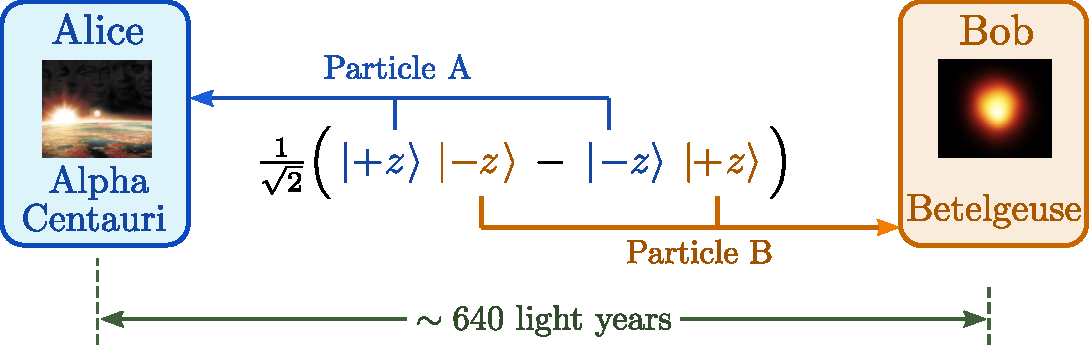
\includegraphics[width=0.75\textwidth]{epr}
\end{figure}

Once ready, Alice measures $\hat{S}_z$ on particle $A$, which induces
an instantaneous collapse of the two-particle state.  Immediately
afterwards, Bob measures $\hat{S}_z$ on particle $B$, and
obtains---with 100\% certainty---the opposite spin.  During the time
interval between these two measurements, no classical signal could
have traveled between the two star systems, not even at the speed of
light.  Yet the state collapse induced by Alice's measurement has a
definite effect on the result of Bob's measurement.

There are three noteworthy aspects of this phenomenon:

First, it dispels some commonsensical but mistaken ``explanations''
for quantum state collapse in terms of perturbative effects.  For
instance, it is sometimes explained that if we want to measure a
particle's position, we need to shine a light beam on it, or disturb
it in some way, and this disturbance generates an uncertainty in the
particle's momentum.  The EPR paradox shows that such stories don't
capture the full weirdness of quantum state collapse, for we can
collapse the state of a particle by doing a measurement on
\textit{another} particle far away!

Second, our experimentalists have a certain amount of control over the
state collapse, due to the choice of what measurement to perform.  So
far, we have considered $S_z$ measurements performed by Alice on
particle $A$.  But Alice can choose to measure the spin of $A$ along
another axis, say $S_x$.  In the basis of spin-up and spin-down
states, the operator $\hat{S}_x$ has matrix representation
\begin{equation}
  \hat{S}_x = \frac{\hbar}{2}\, \begin{pmatrix}0&1\\1&0\end{pmatrix}.
  \end{equation}
The eigenvalues and eigenvectors are
\begin{align}
  \begin{aligned}s_x = \;\;\frac{\hbar}{2},\; &\;\;\; |\!+\!x\rangle = \frac{1}{\sqrt{2}}\Big(|\!+\!z\rangle + |\!-\!z\rangle\Big) \\ s_x = -\frac{\hbar}{2}, &\;\;\; |\!-\!x\rangle = \frac{1}{\sqrt{2}}\Big(|\!+\!z\rangle - |\!-\!z\rangle\Big).\end{aligned}
\end{align}
Conversely, we can write the $\hat{S}_z$ eigenstates in the $\{|\!+\!x\rangle,|\!-\!x\rangle\}$ basis:
\begin{align}
  \begin{aligned}|\!+\!z\rangle &= \frac{1}{\sqrt{2}}\Big(|\!+\!x\rangle + |\!-\!x\rangle\Big) \\ |\!-\!z\rangle &= \frac{1}{\sqrt{2}}\Big(|\!+\!x\rangle - |\!-\!x\rangle\Big).\end{aligned}
\end{align}
This allows us to write the two-particle entangled state in the
$\hat{S}_x$ basis:
\begin{equation}
  |\psi\rangle = \frac{1}{\sqrt{2}} \Big(|\!-\!x\rangle|\!+\!x\rangle \,-\, |\!+\!x\rangle|\!-\!x\rangle\Big).
\end{equation}
Alice's measurement still collapses the particles into definite spin
states with opposite spins---but now spin states of ${S}_x$ rather
than ${S}_z$.

Third, this ability to choose the measurement axis \textit{does not}
allow for superluminal communication.  Alice can choose whether to (i)
measure $S_z$ or (ii) measure $S_x$, and this choice instantaneously
affects the quantum state of particle $B$.  If Bob can find a way to
distinguish between the cases (i) and (ii), even statistically, this
would serve as a method for instantaneous communication, violating the
theory of relativity!  Yet this turns out to be impossible.  The key
problem is that quantum states themselves cannot be measured; only
observables can be measured.  Suppose Alice's measurement is
$\hat{S}_z$, which collapses $B$ to either $|\!+\!z\rangle$ or
$|\!-\!z\rangle$, each with probability $1/2$.  Bob must now choose
which measurement to perform.  If he measures $S_z$, the outcome is
$+\hbar/2$ or $-\hbar/2$ with equal probabilities.  If he measures
$S_x$, the probabilities are:
\begin{align}
  \begin{aligned}P(S_x = +\hbar/2) &= \frac{1}{2}\, \Big|\langle\!+x|\!+\!z\rangle\Big|^2 \;+\;\, \frac{1}{2}\, \Big|\langle\!+x|\!-\!z\rangle\Big|^2 = \frac{1}{2}\\P(S_x = -\hbar/2) &= \frac{1}{2}\, \Big|\langle\!-x|\!+\!z\rangle\Big|^2 \;+\;\, \frac{1}{2}\, \Big|\langle\!-x|\!-\!z\rangle\Big|^2 = \frac{1}{2}.\end{aligned}
\end{align}
The probabilities are still equal!  Repeating this analysis for any
other choice of spin axis, we find that the two possible outcomes
always have equal probability.  Thus, Bob's measurement does not yield
any information about Alice's choice of measurement axis.

Since quantum state collapse does not allow for superluminal
communication, it is consistent \textit{in practice} with the theory
of relativity.  However, state collapse is still \textbf{nonlocal}, in
the sense that unobservable ingredients of the theory (quantum states)
can change faster than light can travel between two points.  For this
reason, EPR argued that quantum theory is \textit{philosophically}
inconsistent with relativity.

EPR suggested an alternative: maybe quantum mechanics is an
approximation of some deeper theory, whose details are currently
unknown, but which is deterministic and local.  Such a
``\textbf{hidden variable theory}'' may give the appearance of
quantum state collapse in the following way.  Suppose each particle
has a definite but ``hidden'' value of $S_z$, either $S_z = +\hbar/2$
or $S_z = -\hbar/2$; let us denote these as $[+]$ or $[-]$.  We can
hypothesize that the two-particle quantum state $|\psi\rangle$ is not
an actual description of reality; rather, it corresponds to a
\textit{statistical} distribution of ``hidden variable'' states,
denoted by $[+;-]$ (i.e., $S_z = +\hbar/2$ for particle $A$ and $S_z =
-\hbar/2$ for particle $B$), and $[-;+]$ (the other way around).

\begin{figure}[h]
  \centering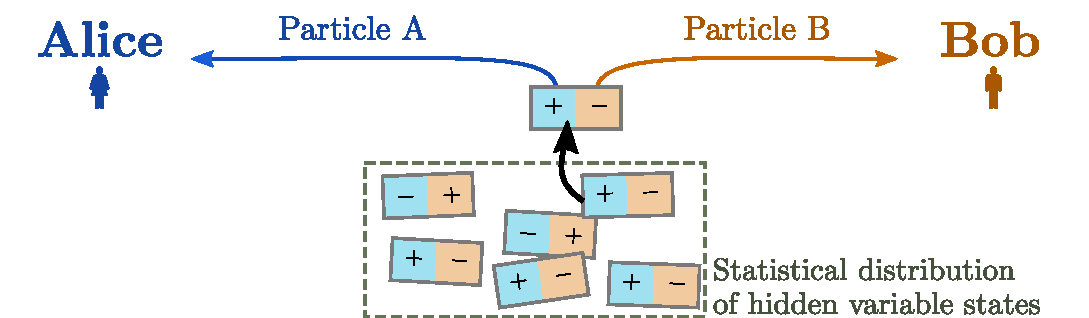
\includegraphics[width=0.75\textwidth]{hiddenvariables}
\end{figure}

When Alice measures $S_z$, the value of the hidden variable is
revealed.  A result of $+z$ implies $[+;-]$, whereas $-z$ implies
$[-;+]$.  When bob subsequently measures $S_z$, the result obtained is
the opposite of Alice's result.  But those were simply the values all
along---there is no instantaneous physical influence traveling between
their two laboratories.

Clearly, there are many missing details in this hypothetical
description.  Any actual hidden variable theory would also need to
replicate the huge list of successful predictions made by quantum
theory.  Trying to come up with a suitable theory of this sort seems
difficult, but with enough hard work, one might imagine that it is
doable.

\section{Bell's theorem}
\label{sec:bell}

In 1964, John S.~Bell published a bombshell paper showing that the
predictions of quantum theory are \textit{inherently inconsistent}
with hidden variable theories [\ref{cite:bell}].  The amazing thing
about this result, known as \textbf{Bell's theorem}, is that it
requires no knowledge about the details of the hidden variable theory,
just that it is deterministic and local.  Here, we present a
simplified version of Bell's theorem due to Mermin
[\ref{cite:mermin}].

We again consider spin-1/2 particle pairs, with particle $A$ sent to
Alice at Alpha Centauri, and particle $B$ to Bob at Betelgeuse.  Each
experimentalist can measure the particle's spin along three distinct
choices of spin axis.  These spin observables are denoted by $S_1$,
$S_2$, and $S_3$.  We will not specify the actual directions of these
spin axes until later in the proof.  For now, just note that the axes
need not correspond to orthogonal spatial directions.

We repeatedly prepare the particle pairs in the singlet state
\begin{equation}
  |\psi\rangle = \frac{1}{\sqrt{2}} \Big(|\!+\!z\rangle|\!-\!z\rangle \,-\, |\!-\!z\rangle|\!+\!z\rangle\Big),
\end{equation}
and send the respective particles to Alice and Bob.  During each round
of the experiment, each experimentalist randomly chooses one of the
three spin axes $S_1$, $S_2$, or $S_3$, and performs that spin
measurement.  It doesn't matter which experimentalist performs the
measurement first; the experimentalists can't influence each other, as
there is not enough time for a light-speed signal to travel between
the two locations.  Many rounds of the experiment are conducted; for
each round, both experimentalists' choices of spin axis are recorded,
along with their measurement results.

\begin{figure}[h]
  \centering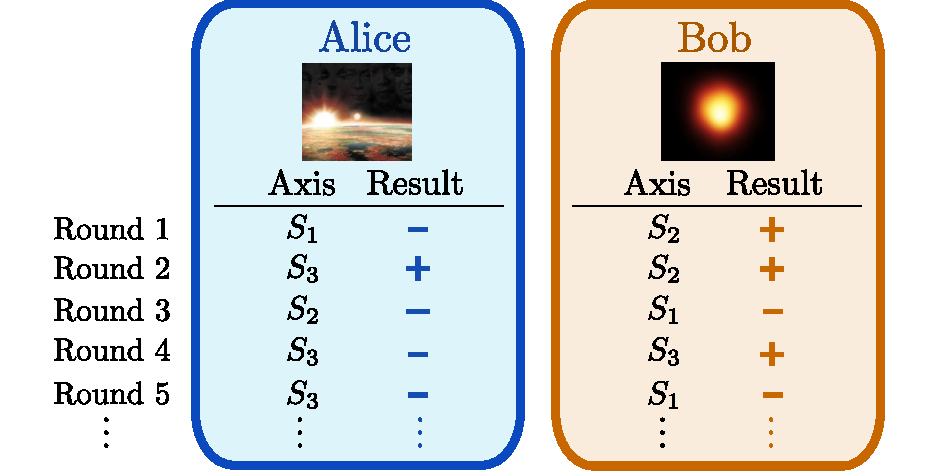
\includegraphics[width=0.67\textwidth]{bell}
\end{figure}

At the end, the experimental records are brought together and
examined.  We assume that the results are consistent with the
predictions of quantum theory.  Among other things, this means that
whenever the experimentalists happen to choose the same measurement
axis, they always find opposite spins.  (For example, this is the case
during ``Experiment 4'' in the above figure, where both
experimentalists happened to measure $S_3$.)

Can a hidden variable theory reproduce the results predicted by
quantum theory?  In a hidden variable theory, each particle must have
a definite value for each spin observable.  For example, particle $A$
might have $S_1 = +\hbar/2, \, S_2 = +\hbar/2, \, S_3 = -\hbar/2$.
Let us denote this by $[++-]$.  To be consistent with the predictions
of quantum theory, the hidden spin variables for the two particles
must have opposite values along each direction.  This means that there
are $8$ distinct possibilities, which we can denote as
\begin{align*}
  \begin{aligned}{[}{+++};{---}], \;\;\; [{++-};{--+}], \;\;\; [{+-+};{-+-}], \;\;\; [{+--};{-++}],\\ [{-++};{+--}], \;\;\; [{-+-};{+-+}], \;\;\; [{--+};{++-}], \;\;\; [{---};{+++}].\end{aligned}
\end{align*}
For instance, $[{++-};{--+}]$ indicates that for particle $A$, $S_1 =
S_2 = +\hbar/2$ and $S_3 = -\hbar/2$, while particle $B$ has the
opposite spin values, $S_1 = S_2 = -\hbar/2$ and $S_3 = +\hbar/2$.
So far, however, we don't know anything about the relative
probabilities of these 8 cases.

Let's now focus on the subset of experiments in which the two
experimentalists happened to choose \textit{different} spin axes
(e.g., Alice chose $S_1$ and Bob chose $S_2$).  Within this subset,
what is the probability \textit{for the two measurement results to
  have opposite signs} (i.e., one $+$ and one $-$)?  To answer this
question, we first look at the following 6 cases:
\begin{align*}
  \begin{aligned}{[}{++-};{--+}], \;\;\; [{+-+};{-+-}], \;\;\; [{+--};{-++}],\\ [{-++};{+--}], \;\;\; [{-+-};{+-+}], \;\;\; [{--+};{++-}].\end{aligned}
\end{align*}
These are the cases which do not have all $+$ or all $-$ for each
particle.  Consider one of these, say ${[}{++-};{--+}]$.  The two
experimentalists picked their measurement axes at random each time,
and amongst the experiments where they picked different axes, there
are two ways for the measurement results to have opposite signs:
$(S_1,S_2)$ or $(S_2,S_1)$.  There are four ways to get the same sign:
$(S_1,S_3)$, $(S_2,S_3)$, $(S_3,S_1)$ and $(S_3, S_2)$.  Thus,
for this particular set of hidden variables, the probability for
measurement results with opposite signs is 1/3.  If we go through all
6 of the cases listed above, we find that in call cases, the
probability for opposite signs is 1/3.

Now look at the remaining 2 cases:
\begin{equation*}
  {[}{+++};{---}], \;\;\; [{---};{+++}].
\end{equation*}
For these, Alice and Bob always obtain results with opposite signs.
Combining this with the findings from the previous paragraph, we
obtain the following statement:

\textit{Given that the two experimentalists choose different spin
  axes, the probability that their results have opposite signs is $P
  \ge 1/3$.}

This is called \textbf{Bell's inequality}.  If we can arrange a
situation where quantum theory predicts a probability $P < 1/3$ (i.e.,
a violation of Bell's inequality), that would mean that quantum theory
is inherently inconsistent with local deterministic hidden variables.
This conclusion would hold regardless of the ``inner workings'' of the
hidden variable theory.  In particular, note that the above derivation
made no assumptions about the relative probabilities of the hidden
variable states.

To complete the proof, we must find a set $\{S_1, S_2, S_3\}$ such
that the predictions of quantum mechanics violate Bell's inequality.
One simple choice is to align $S_1$ with the $z$ axis, and align $S_2$
and $S_3$ along the $x$-$z$ plane at $120^\circ$ ($2\pi/3$ radians)
from $S_1$, as shown below:

\begin{figure}[h]
  \centering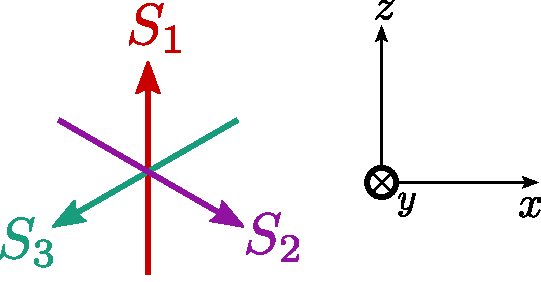
\includegraphics[width=0.28\textwidth]{bellaxes}
\end{figure}

The corresponding spin operators can be written in the eigenbasis of
$\hat{S}_z$:
\begin{align}
  \begin{aligned}\hat{S}_1 &= \frac{\hbar}{2} \, \sigma_3 \\ \hat{S}_2 &= \frac{\hbar}{2} \, \left[\cos(2\pi/3) \sigma_3 + \sin(2\pi/3)\sigma_1\right]  \\   \hat{S}_3 &= \frac{\hbar}{2} \, \left[\cos(2\pi/3) \sigma_3 - \sin(2\pi/3)\sigma_1\right].\end{aligned}
\end{align}

Suppose Alice chooses $S_1$, and obtains $+\hbar/2$.  Particle $A$
collapses to state $|\!+\!z\rangle$, and particle $B$ collapses to
state $|\!-\!z\rangle$.  Bob is assumed to choose a different spin
axis.  If the choice is $S_2$, the expectation value is
\begin{align}
  \begin{aligned}\langle\, - z \, | \, S_2 \,|-\!z\,\rangle &= \frac{\hbar}{2} \Big[\cos(2\pi/3) \langle\,- z\,|\sigma_3| - \!z\,\rangle + \sin(2\pi/3)\langle\,- z\,|\sigma_1|-\!z\,\rangle\Big]\\ &= \frac{\hbar}{2} \cdot \frac{1}{2} \end{aligned}
\end{align}
If $P_+$ and $P_-$ respectively denote the probability of measuring
$+\hbar/2$ and $-\hbar/2$ in this measurement, the above equation
implies that $P_+ - P_- = + 1/2$.  Moreover, $P_+ + P_- = 1$ by
probability conservation.  Hence, the probability of obtaining a
negative value (the opposite sign from Alice's measurement) is $P_- =
1/4$.  All the other possible scenarios are worked out similarly.  The
result is that the overall probability of the two experimentalists
obtaining opposite results (in the cases where they choose different
measurement axis) is $1/4$.  Bell's inequality is violated!

Last of all, we must consult Nature itself.  Is it possible to
observe, in an actual experiment, probabilities that violate Bell's
inequality?  In the decades following Bell's 1964 paper, many
experiments were performed to answer this question.  These experiments
are all substantially more complicated than the simple two-particle
spin-$1/2$ model that we've studied, and they are subject to various
uncertainties and ``loopholes'' that are beyond the scope of our
discussion.  But in the end, the experimental consensus appears to be
a clear \textit{yes}: Nature really does behave according to quantum
mechanics, and in a manner that cannot be replicated by deterministic
local hidden variables!  A summary of the experimental evidence is
given in a review paper by Aspect [\ref{cite:aspect}].

\section{Quantum cryptography}

One of the most remarkable consequences of Bell's thought experiment
is that it provides a way to perform cryptography that is more secure,
in certain respects, than conventional cryptography.  The possibility
of \textbf{quantum cryptography}, first raised by Ekert
[\ref{cite:ekert}], is poised to be one of the most important
technological applications of quantum mechanics.

Ekert's quantum cryptography scheme allows two participants, Alice and
Bob, to share with each other a string of random binary digits (0 or
1), called a ``key'', in such a manner that no one else can learn the
key by eavesdropping on their communications.  Once Alice and Bob have
established a secret shared key, it can be used to encrypt subsequent
messages between them, which nobody else can decipher (e.g., by using
\href{https://en.wikipedia.org/wiki/One-time_pad}{one-time pads}).

The scheme follows almost immediately from the Bell thought experiment
of Section \ref{sec:bell}.  In each round, a pair of spin-$1/2$
particles is prepared in the singlet state, with particle $A$ sent to
Alice and $B$ sent to Bob.  Alice and Bob each randomly choose a
measurement axis ($S_1$, $S_2$, or $S_3$), and measure the spin of
their particle along that axis.

After an appropriate number of rounds, Alice and Bob publicly announce
their choices of measurement axes.  These announcements are assumed to
take place over a classical communication channel that cannot be
jammed or manipulated by any hostile party (though it can be
eavesdropped upon).  From the announcements, Alice and Bob determine
the rounds in which they happened to pick the same axes.  Their
measurement results during these rounds are guaranteed to be the
opposites of each other.  Hence, they have established a random binary
string known to each other but to no one else.

How might an eavesdropper, Eve, attempt to foil this scheme?  Suppose
Eve can intercept some or all of the particles $B$ destined for Bob.
She might try to substitute her own measurements, in a manner that
could let her work out the secret key.  However, Eve is hampered by
the fact that she is unable to predict or influence Bob's choices of
measurement axes (i.e., Bob's choices are truly random), nor is she
able to impersonate Bob during the announcements of the axis choices
(i.e., the classical communication channel is unjammable).  Under
these assumptions, it can be shown that any attempt by Eve to
substitute her own measurements can be detected by Alice and Bob, by
performing a statistical analysis of their measurement results in the
rounds with different different axis choices.  The detection of the
eavesdropper turns out to be essentially the same as checking for
Bell's inequality.  For details, refer to Ref.~[\ref{cite:ekert}].

Alternatively, Eve might try to ``clone'' the quantum state of
particle $B$ before passing it along to Bob.  If this can be done, Eve
can retain the cloned quantum state, wait for Bob to announce his
choice of measurement axis for that round, and then perform the
corresponding measurement to reproduce Bob's result.  Though plausible
at first glance, this turns out to be fundamentally unworkable, as it
is incompatible with the laws of quantum mechanics.

The so-called \textbf{no-cloning theorem} can be proven as follows.
Eve desires to clone an arbitrary state of a spin-half particle $B$
onto another spin-half particle $C$.  The two-particle Hilbert space
is $\mathscr{H}\otimes\mathscr{H}$.  With particle $C$ initially
prepared in some state $|0\rangle$, Eve must devise a unitary
operation $\hat{U}$, representing the cloning process, such that
\begin{equation}
  \hat{U} |\psi\rangle | 0\rangle = e^{i\phi} |\psi\rangle |\psi\rangle
  \label{clone}
\end{equation}
for all $|\psi\rangle \in \mathscr{H}$, and for some phase factor
$\phi$ that could depend on $|\psi\rangle$.  Note that the value of
$\phi$ does not affect the outcomes of measurements.

Now replace $|\psi\rangle$ in the above equation with two arbitrary
states denoted by $|\psi_1\rangle$ and $|\psi_2\rangle$, and take
their inner product.  According to Eq.~\eqref{clone},
\begin{align}
  \Big(\langle \psi_1 | \langle 0 | \hat{U}^\dagger \Big)
  \Big(\hat{U} | \psi_2 \rangle |0\rangle \Big)
  &=  \Big(\langle \psi_1| \langle \psi_1| e^{-i\phi_1} \Big) \Big( e^{i\phi_2} |\psi_2\rangle|\psi_2\rangle\Big) \\
  &= e^{-i(\phi_1-\phi_2)} \Big( \langle\psi_1 | \psi_2\rangle \Big)^2. \label{clone1}
\end{align}
Here, $\phi_1$ and $\phi_2$ are the phase factors from
Eq.~\eqref{clone} for the two chosen states.  On the other hand, since
$\hat{U}$ is unitary,
\begin{align}
  \langle \psi_1 | \langle 0 | \hat{U}^\dagger \hat{U} | \psi_2 \rangle |0\rangle
  &= \Big(\langle \psi_1 | \langle 0| \Big) \Big(| \psi_2 \rangle |0\rangle\Big)
  \\ &= \langle\psi_1 | \psi_2\rangle. \label{clone2}
\end{align}
Here we have used the fact that $\langle 0 | 0\rangle = 1$.  Comparing
the magnitudes of \eqref{clone1} and \eqref{clone2},
\begin{equation}
  \big|\langle \psi_1 | \psi_2\rangle \big|^2
  = \big| \langle\psi_1 | \psi_2\rangle \big|
  \;\;\Rightarrow \;\;
  \big|\langle\psi_1 | \psi_2\rangle\big| = 0 \;\mathrm{or}\; 1.
\end{equation}
But aside from the trivial case of a one-dimensional Hilbert space,
this cannot be true for arbitrary $|\psi_1\rangle$ and
$|\psi_2\rangle$.  For instance, for a two-dimensional space spanned
by an orthonormal basis $\{|0\rangle, |1\rangle\}$, we can pick
\begin{equation}
  |\psi_1\rangle = |0\rangle, \;
  |\psi_2\rangle = \frac{1}{\sqrt{2}}\big(|0\rangle +
  |1\rangle\big)
  \;\;\Rightarrow\;\;
  \big|\langle\psi_1|\psi_2\rangle\big| = \frac{1}{\sqrt{2}}.
\end{equation}

\clearpage
\section{Density operators}

We now introduce the \textbf{density operator}, which helps to
streamline many calculations in multi-particle quantum mechanics.

Consider a quantum system with a $d$-dimensional Hilbert space
$\mathscr{H}$.  Given an arbitrary state $|\psi\rangle \in
\mathscr{H}$, define
\begin{equation}
  \hat{\rho} = |\psi\rangle\, \langle\psi|.
  \label{rho_pure}
\end{equation}
This is just the projection operator for $|\psi\rangle$, but in this
context we call it a ``density operator''.  Some other authors call it
a \textbf{density matrix}, based on the fact that linear operators can
be represented as matrices.  It has the following noteworthy features:

\begin{enumerate}
\item It is Hermitian.  

\item Suppose $\hat{Q}$ is an observable with eigenvalues $\{q_\mu\}$
  and eigenstates $\{|\mu\rangle\}$ (where $\mu$ is some label that
  enumerates the eigenstates.  If we do a $\hat{Q}$ measurement on
  $|\psi\rangle$, the probability of obtaining $q_\mu$ is
  \begin{equation}
    P_\mu = \big|\langle \mu | \psi\rangle\big|^2 =
    \langle \mu |\, \hat{\rho}\, | \mu \rangle.
    \label{Pi_rho}
  \end{equation}

\item Moreover, the expectation value of the observable is
  \begin{equation}
    \langle Q\rangle
    = \sum_\mu q_\mu P_\mu
    = \sum_\mu q_\mu \langle \mu | \hat{\rho}| \mu \rangle
    = \mathrm{Tr}\big[\,\hat{Q} \, \hat{\rho}\,\big].
    \label{Qexpt}
  \end{equation}
  In the last equality, $\mathrm{Tr}[\cdots]$ denotes the trace, which
  is the sum of the diagonal elements of the matrix representation of
  the operator.  The value of the trace is basis-independent.
\end{enumerate}

Now consider, once again, a composite system consisting of two
subsystems $A$ and $B$, with Hilbert spaces $\mathscr{H}_A$ and
$\mathscr{H}_B$.  Let's say we are interested in the physical behavior
of $A$, that is to say the outcome probabilities and expectation
values of any measurements performed on $A$.  These can be calculated
from $|\psi\rangle$, the state of the combined system; however,
$|\psi\rangle$ also carries information about $B$, which is not
relevant to us as we only care about $A$.

There is a more economical way to encode just the information about
$A$.  We can define the density operator for subsystem $A$ (sometimes
called the \textbf{reduced density operator}):
\begin{equation}
  \hat{\rho}_A = \mathrm{Tr}_B \,\big[\,\hat{\rho}\,\big].
  \label{rhoa_def}
\end{equation}
Here, $\mathrm{Tr}_B[\cdots]$ refers to a \textbf{partial trace}.
This means tracing over the $\mathscr{H}_B$ part of the Hilbert space
$\mathscr{H} = \mathscr{H}_A \otimes \mathscr{H}_B$, which yields an
operator acting on $\mathscr{H}_A$.

To better understand Eq.~\eqref{rhoa_def}, let us go to an explicit
basis.  Let $\hat{Q}_A$ be an observable for $\mathscr{H}_A$ with
eigenbasis $\{|\mu\rangle\}$, and let $\hat{Q}_B$ be an observable for
$\mathscr{H}_B$ with eigenbasis $\{|\nu\rangle\}$.  If the density
operator of the combined system is $\hat{\rho} = |\psi\rangle\langle
\psi|$, then
\begin{equation}
  \hat{\rho}_A =
    \sum_\nu
    \Big( \hat{I}\otimes \langle \nu| \Big)
    \; |\psi\rangle \langle \psi | \;
    \Big( \hat{I}\otimes | \nu\rangle \Big).
    \label{rhoa_explicit}
\end{equation}
This is a Hermitian operator acting on the $\mathscr{H}_A$ space.  In
the $\{|\mu\rangle\}$ basis, its diagonal matrix elements are
\begin{align}
  \begin{aligned}
    \langle \mu | \hat{\rho}_A | \mu \rangle
    &=
    \sum_\nu
    \Big( \langle \mu| \langle \nu| \Big)
    \, |\psi\rangle \langle \psi | \,
    \Big( |\mu\rangle | \nu\rangle \Big) \\
    &=
    \langle \psi | \,
    \left[ |\mu\rangle \langle \mu| \otimes
      \left(\sum_\nu | \nu\rangle \langle \nu|\right) \right]
    |\psi\rangle \\
    &=
    \langle \psi | \,
    \Big( |\mu\rangle \langle \mu| \otimes \hat{I}_B\Big) |\psi\rangle.
  \end{aligned}
\end{align}
According to the rules of partial measurements discussed in
Section~\ref{sec:partialmeasurements}, this is precisely the
probability of obtaining $q_\mu$ when measuring $\hat{Q}_A$ on subsystem
$A$:
\begin{equation}
  P_\mu = \langle \mu | \hat{\rho}_A | \mu \rangle.
  \label{rho_prob}
\end{equation}
It follows that the expectation value for observable $\hat{M}$ is
\begin{equation}
  \langle Q_A \rangle = \sum_\mu q_\mu
  \langle \mu | \hat{\rho}_A | \mu \rangle
  = \mathrm{Tr}\Big[\hat{Q}_A \, \hat{\rho}_A \Big].
  \label{rho_expect}
\end{equation}
These results hold for any choice of basis.  Hence, knowing the
density operator for $A$, we can determine the outcome probabilities
of \textit{any} partial measurement performed on $A$.

To better understand the properties of $\hat{\rho}_A$, let us write
$|\psi\rangle$ explicitly as
\begin{equation}
  |\psi\rangle = \sum_{\mu\nu} \psi_{\mu\nu} |\mu\rangle |\nu\rangle,
\end{equation}
where $\sum_{\mu\nu} |\psi_{\mu\nu}|^2 = 1$.  Then
\begin{align}
  \begin{aligned}
    \hat{\rho} &= \sum_{\mu\mu'\nu\nu'} \psi_{\mu\nu}
    \psi_{\mu'\nu'}^* \; |\mu\rangle |\nu\rangle \,
    \langle\mu'|\langle \nu'| \\
    \hat{\rho}_A &= \sum_{\mu\mu'\nu} \psi_{\mu\nu}\psi_{\mu'\nu}^* |\mu\rangle
    \langle\mu'| \\
    &= \sum_\nu \left(\sum_\mu \psi_{\mu\nu} |\mu\rangle\right)
    \left(\sum_{\mu'} \psi_{\mu'\nu}^*\langle\mu'|\right) \\
    &= \sum_\nu |\varphi_\nu\rangle \langle \varphi_\nu|,
    \;\;\;\mathrm{where}\;\;\;
    |\varphi_\nu\rangle = \sum_\mu \psi_{\mu\nu} |\mu\rangle.
  \end{aligned}
\end{align}
But $|\varphi_\nu\rangle$ is not necessarily normalized to unity:
$\langle \varphi_\nu | \varphi_\nu\rangle =
\sum_{\mu}|\psi_{\mu\nu}|^2 \le 1$.  Let us define
\begin{equation}
  |\tilde{\varphi}_\nu\rangle = \frac{1}{\sqrt{P_\nu}} |\varphi_\nu\rangle,
  \;\;\;\mathrm{where} \;\; P_\nu = \sum_{\mu}|\psi_{\mu\nu}|^2.
\end{equation}
Note that each $P_\nu$ is a non-negative real number in the range
$[0,1]$.  Then
\begin{equation}
  \hat{\rho}_A = \sum_\nu P_\nu\, |\tilde{\varphi}_\nu\rangle
  \langle \tilde{\varphi}_\nu|,
  \;\;\;\mathrm{where}\;\;
  \begin{cases}
    \;\;\textrm{each $P_\nu$ is a real number in $[0,1]$, and} \\
    \;\;\textrm{each}\; |\tilde{\varphi}_\nu\rangle \in \mathscr{H}_A,
    \;\;\mathrm{with}
    \;\;\langle\tilde{\varphi}_\nu|\tilde{\varphi}_\nu\rangle = 1.
  \end{cases}
  \label{rhoform}
\end{equation}

In general, we can define a density operator as any operator that has
the form of Eq.~\eqref{rhoform}, regardless of whether or not it was
formally derived via a partial trace.  We can interpret it as
describing a ensemble of quantum states weighted by a set of classical
probabilities.  Each term in the sum consists of (i) a weighting
coefficient $P_\nu$ which can be regarded as a probability (the
coefficients are all real numbers in the range $[0,1]$, and sum to 1),
and (ii) a projection operator associated with some normalized state
vector $|\tilde{\varphi}_\nu\rangle$.  Note that the states in the
ensemble do not have to be orthogonal to each other.

From this point of view, a density operator of the form
$|\psi\rangle\langle\psi|$ corresponds to the special case of an
ensemble containing only one quantum state $|\psi\rangle$.  Such an
ensemble is called a \textbf{pure state}, and describes a quantum
system that is not entangled with any other system.  If an ensemble is
not a pure state, we call it a \textbf{mixed state}; it describes a
system that is entangled with some other system.

We can show that any linear operator $\hat{\rho}_A$ obeying
Eq.~\eqref{rhoform} has the following properties:
\begin{enumerate}
\item $\hat{\rho}_A$ is Hermitian.

\item $\langle\varphi|\hat{\rho}_A|\varphi\rangle \ge 0$ for any
  $|\varphi\rangle \in \mathscr{H}_A$ (i.e., the operator is positive
  semidefinite).

\item For any observable $\hat{Q}_A$ acting on $\mathscr{H}_A$,
  \begin{align}
    \begin{aligned}
      \langle Q_A \rangle
      &\equiv \sum_\nu P_\nu
      \langle \tilde{\varphi}_\nu|\hat{Q}_A|\tilde{\varphi}_\nu\rangle \\
      &= \sum_{\mu\nu} P_\nu\,
      \langle \tilde{\varphi}_\nu|\mu\rangle \,
      \langle\mu|\hat{Q}|\tilde{\varphi}_\nu\rangle
      \;\;\;\big(\textrm{using some basis} \;\{|\mu\rangle\}\big) \\
      &= \sum_\mu
      \langle\mu|\hat{Q} \left(\sum_\nu |\tilde{\varphi}_\nu\rangle
      \langle \tilde{\varphi}_\nu|\right) |\mu\rangle \\
      &= \mathrm{Tr}\left[\,\hat{Q} \,\hat{\rho}_A\,\right].
    \end{aligned}
    \label{prop3}
  \end{align}
  This property can be used to deduce the probability of obtaining any
  measurement outcome: if $|\mu\rangle$ is the eigenstate associated
  with the outcome, the outcome probability is
  $\langle\mu|\hat\rho_A|\mu\rangle$, consistent with
  Eq.~\eqref{rho_prob}.  To see this, take $\hat{Q} = |\mu\rangle
  \langle \mu|$ in Eq.~\eqref{prop3}.
  
\item The eigenvalues of $\hat{\rho}_A$, denoted by $\{p_1, p_2,
  \dots, p_{d_A}\}$, satisfy
  \begin{equation}
    p_j \in \mathbb{R} \;\;\;\mathrm{and}\;\; 0 \le p_j \le 1 \;\;
    \mathrm{for}\;\; j = 1,\dots,d_A,
    \quad\mathrm{with}\;\; \sum_{j=1}^{d_A} p_j = 1.
    \label{trrho_reduced}    
  \end{equation}
  In other words, the eigenvalues can be interpreted as probabilities.
  This also implies that $\mathrm{Tr}[\hat\rho_A] = 1$.

  This property follows from Property 3 by taking $\hat{Q} =
  |\varphi\rangle\langle\varphi|$, where $|\varphi\rangle$ is any
  eigenvector of $\hat\rho_A$, and then taking $\hat{Q} = \hat{I}_A$.
\end{enumerate}

\section{Entanglement entropy}
\label{sec:entropy}

Previously, we said that a multi-particle system is entangled if the
individual particles lack definite quantum states.  It would be nice
to make this statement more precise, and in fact physicists have come
up with several different quantitive measures of entanglement.  In
this section, we will describe the most common measure,
\textbf{entanglement entropy}, which is closely related to the entropy
concept from thermodynamics, statistical mechanics, and information
theory.

We have seen from the previous section that if a subsystem $A$ is
(possibly) entangled with some other subsystem $B$, the information
required to calculate all partial measurement outcomes on $A$ is
stored within a reduced density operator $\hat{\rho}_A$.  We can use
this to define a quantity called the \textbf{entanglement entropy} of
$A$:
\begin{equation}
  S_{A} = - k_b \, \mathrm{Tr}_A \Big\{ \hat{\rho}_A\, \ln\!\big[\hat{\rho}_A\big]\Big\}.
  \label{entropy}
\end{equation}
In this formula, $\ln[\cdots]$ denotes the logarithm of an operator,
which is the inverse of the exponential: $\ln(\hat{P}) = \hat{Q}
\Rightarrow \exp(\hat{Q}) = \hat{P}$.  The prefactor $k_b$ is
Boltzmann's constant, and ensures that $S_A$ has the same units as
thermodynamic entropy.

The definition of the entanglement entropy is based on an analogy with
the entropy concept from classical thermodynamics, statistical
mechanics and information theory.  In those classical contexts,
entropy is a quantitative measure of uncertainty (i.e, lack of
information) about a system's underlying microscopic state, or
``microstate''.  Suppose a system has $W$ possible microstates that
occur with probabilities $\{p_1, p_2, \dots, p_W\}$, satisfying
$\sum_i p_i = 1$.  Then we define the classical entropy
\begin{equation}
  S_{\mathrm{cl.}} = - k_b \sum_{i=1}^W p_i \ln(p_i).
\end{equation}
In a situation of complete certainty where the system is known to be
in a specific microstate $k$ ($p_i = \delta_{ik}$), the formula gives
$S_{\mathrm{cl.}} = 0$.  (Note that $x \ln(x)\rightarrow 0$ as
$x\rightarrow 0$).  In a situation of complete uncertainty where all
microstates are equally probable ($p_i = 1/W$), we get
$S_{\mathrm{cl.}} = k_b \ln W$, the entropy of a microcanonical
ensemble in statistical mechanics.  For any other distribution of
probabilities, it can be shown that the entropy lies between these two
extremes: $0 \le S_{\mathrm{cl.}}  \le k_b\ln W$.  For a review of the
properties of entropy, see Appendix C.

The concept of entanglement entropy aims to quantify the uncertainty
arising from a quantum (sub)system's lack of a definite quantum state,
due to it being possibly entangled with another (sub)system.  When
formulating it, the key issue we need to be careful about is how to
extend classical notions of probability to quantum systems.  We have
seen that when performing a measurement on $A$ whose possible outcomes
are $\{q_\mu\}$, the probability of getting $q_\mu$ is $P_\mu =
\langle \mu | \hat{\rho}_A|\mu\rangle$.  However, it is problematic to
directly substitute these probabilities $\{P_\mu\}$ into the classical
entropy formula, since they are basis-dependent (i.e., the set of
probabilities is dependent on the choice of measurement).
Eq.~\eqref{entropy} bypasses this problem by using the trace, which is
basis-independent.

In the special case where $\{|\mu\rangle\}$ is the eigenbasis for
$\hat{\rho}_A$, the connection is easier to see.  From
\eqref{trrho_reduced}, the eigenvalues $\{p_\mu\}$ are all real numbers
between 0 and 1, and summing to unity, so they can be regarded as
probabilities.  Then the entanglement entropy is
\begin{align}
  \begin{aligned}
    S_A &= -k_b \sum_\mu \langle \mu | \hat{\rho}_A \ln(\hat{\rho}_A) | \mu\rangle  \\
    &= - k_b \sum_\mu p_\mu \ln(p_\mu).
  \end{aligned}
\end{align}
Therefore, in this particular basis the expression for the
entanglement entropy is consistent with the classical definition of
entropy, with the eigenvalues of $\hat{\rho}_A$ serving as the
relevant probabilities.

By analogy with the classical entropy formula (see Appendix C), the
entanglement entropy has the following bounds:
\begin{equation}
  0 \le S_A \le k_b\ln(d_A),
  \label{Sabounds}
\end{equation}
where $d_A$ is the dimension of $\mathscr{H}_A$.

The lower bound $S_A = 0$ holds if and only if system $A$ is in a pure
state (i.e., it is not entangled with any other system).  This is
because the bound corresponds to a situation where $\hat{\rho}_A$ has
one eigenvalue that is 1, and all the other eigenvalues are 0 (see
Appendix C).  If we denote the eigenvector associated with the
non-vanishing eigenvalue by $|\psi\rangle$, then the density matrix
can be written as $\hat{\rho}_A = |\varphi\rangle\langle\varphi|$, which
has the form of a pure state.

As a corollary, if we find that $S_{A} \ne 0$, then $\hat{\rho}_A$
cannot be written as a pure state $|\psi\rangle\langle\psi|$ for
\textit{any} $|\psi\rangle$, and hence it must describe a mixed state.

A system is said to be \textbf{maximally entangled} if it saturates
the upper bound of \eqref{Sabounds}, $S_A = k_b \ln(d_A)$.  This
occurs if and only if the eigenvalues of the density operator are all
equal: i.e., $p_j = 1/d_A$ for all $j = 1, \dots, d_A$.

\begin{framed}
\noindent
\textit{Example}---Consider the following state of two spin-$1/2$
particles:
\begin{align}
  |\psi\rangle = \frac{1}{\sqrt{2}} \Big(|\!+\!z\rangle|\!-\!z\rangle \,-\, |\!-\!z\rangle|\!+\!z\rangle\Big).
\end{align}
The density operator for the two-particle system is
\begin{equation}
  \hat{\rho}(\psi) = \frac{1}{2} \Big(|\!+\!z\rangle|\!-\!z\rangle \,-\, |\!-\!z\rangle|\!+\!z\rangle\Big) \Big(\langle+z|\langle-z| \,-\, \langle-z|\langle+z|\Big).
\end{equation}
Tracing over system $B$ (the second slot) yields the reduced density operator
\begin{equation}
  \hat{\rho}_A(\psi) = \frac{1}{2} \Big(|\!+\!z\rangle \langle+z| \,+\, |\!-\!z\rangle \langle-z|\Big).
\end{equation}
This can be expressed as a matrix in the
$\{|\!+z\rangle,|\!-z\rangle\}$ basis:
\begin{equation}
  \hat{\rho}_A(\psi) = \begin{pmatrix}\frac{1}{2} & 0 \\ 0 & \frac{1}{2}\end{pmatrix}.
\end{equation}
Now we can use $\hat{\rho}_A$ to compute the entanglement entropy
\begin{equation}
  S_A = -k_b\mathrm{Tr}\left\{\hat{\rho}_A\ln(\rho_A)\right\} = -k_b\mathrm{Tr}\begin{pmatrix}\frac{1}{2}\ln\left(\frac{1}{2}\right) & 0 \\ 0 & \frac{1}{2}\ln\left(\frac{1}{2}\right)\end{pmatrix} = k_b\ln(2).
\end{equation}
Hence, the particles are maximally entangled.
\end{framed}

\section{The Many Worlds Interpretation}

We conclude this chapter by discussing a set of compelling but
controversial ideas arising from the phenomenon of quantum
entanglement: the \textbf{Many Worlds Interpretation} as formulated by
Hugh Everett [\ref{cite:everett}].

So far, when describing the phenomenon of state collapse, we have
relied on the measurement postulate (see
Section~\ref{sec:partialmeasurements}), which is part of the
\textbf{Copenhagen Interpretation} of quantum mechanics.  This is how
quantum mechanics is typically taught, and how physicists think about
the theory when doing practical, everyday calculations.

However, the measurement postulate has two bad features:

\begin{enumerate}
\item It stands apart from the other postulates of quantum mechanics,
  for it is the only place where randomness (or ``indeterminism'')
  creeps into quantum theory.  The other postulates do not refer to
  probabilities.  In particular, the Schr\"odinger equation
\begin{equation}
  i\hbar\frac{\partial}{\partial t}|\psi(t)\rangle = \hat{H}(t) |\psi(t)\rangle
\end{equation}
is completely deterministic.  If you know $\hat{H}(t)$ and are given
the state $|\psi(t_0)\rangle$ at some time $t_0$, you can in principle
determine $|\psi(t)\rangle$ for all $t$.  This time-evolution consists
of a smooth, non-random rotation of the state vector within its
Hilbert space.  A measurement process, however, has a completely
different character: it causes the state vector to jump
discontinuously to a randomly-selected value.  It is strange that
quantum theory contains two completely different ways for a state to
change.

\item The measurement postulate is silent on what constitutes a
measurement.  Does measurement require a conscious observer?  Surely
not: as Einstein once exasperatedly asked, are we really expected to
believe that the Moon exists only when we look at it?  But if a given
device interacts with a particle, what determines whether it acts via
the Schr\"odinger equation, or performs a measurement?
\end{enumerate}

The Many Worlds Interpretation seeks to resolve these problems by
positing that \textit{the measurement postulate is \underline{not} a
  fundamental postulate of quantum mechanics}.  Rather, what we call
``measurement'', including state collapse and the apparent randomness
of measurement results, is an emergent phenomenon that can be derived
from the behavior of complex many-particle quantum systems obeying the
Schr\"odinger equation.  The key idea is that a measurement process
can be described by applying the Schr\"odinger equation to a quantum
system containing both the thing being measured \textit{and} the
measurement apparatus itself.

We can study this using a toy model formulated by Albrecht
[\ref{cite:albrecht}].  Consider a spin-$1/2$ particle, and an
apparatus designed to measure $S_z$.  Let $\mathscr{H}_S$ be the
spin-$1/2$ Hilbert space (which is 2D), and $\mathscr{H}_A$ be the
Hilbert space of the apparatus (which has dimension $d$).  We will
assume that $d$ is very large, as actual experimental apparatuses are
macroscopic objects containing $10^{23}$ or more atoms!  The Hilbert
space of the combined system is
\begin{equation}
  \mathscr{H} = \mathscr{H}_S \otimes \mathscr{H}_A,
\end{equation}
and is $2d$-dimensional.  Let us suppose the system is prepared in an initial
state
\begin{equation}
  |\psi(0)\rangle = \Big(a_+ |\!+z\rangle + a_- |\!-z\rangle\Big) \otimes |\Psi\rangle,
\end{equation}
where $a_\pm\in\mathbb{C}$ are the quantum amplitudes for the particle
to be initially spin-up or spin-down, and $|\Psi\rangle \in
\mathscr{H}_A$ is the initial state of the apparatus.

The combined system now evolves via the Schr\"odinger equation.  We
aim to show that if the Hamiltonian has the form
\begin{equation}
  \hat{H} = \hat{S}_z \otimes \hat{V},
\end{equation}
where $\hat{S}_z$ is the operator corresponding to the observable
$S_z$, then time evolution has an effect equivalent to the measurement
of $S_z$.

It turns out that we can show this without making any special choices
for $\hat{V}$ or $|\Psi\rangle$.  We only need $d \gg 2$, and for both
$\hat{V}$ and $|\Psi\rangle$ to be ``sufficiently complicated''.  We
choose $|\Psi\rangle$ to be a random state vector, and choose random
matrix components for the operator $\hat{V}$.  The precise generation
procedures will be elaborated on later.  Once we decide on
$|\Psi\rangle$ and $\hat{V}$, we can evolve the system by solving the
Sch\"odinger equation
\begin{equation}
  |\psi(t)\rangle = U(t)|\psi(0)\rangle, \;\;\;\mathrm{where}\;\; \hat{U}(t) = \exp\left[-\frac{i}{\hbar}\hat{H}t\right].
\end{equation}
Because the part of $\hat{H}$ acting on the $\mathscr{H}_S$ subspace
is $\hat{S}_z$, the result necessarily has the following form:
\begin{align}
  \begin{aligned}|\psi(t)\rangle &= \hat{U}(t)\Big(a_+ |\!+\!z\rangle + a_- |\!-\!z\rangle\Big) \otimes |\Psi\rangle \\ &= a_+ |\!+\!z\rangle \otimes |\Psi_+(t)\rangle \;+\; a_- |\!-\!z\rangle \otimes |\Psi_-(t)\rangle. \end{aligned}
\end{align}
Here, $|\Psi_+(t)\rangle$ and $|\Psi_-(t)\rangle$ are apparatus states
that are ``paired up'' with the $|\!+\!z\rangle$ and $|\!-\!z\rangle$
states of the spin-$1/2$ subsystem.  At $t=0$, both
$|\Psi_+(t)\rangle$ and $|\Psi_-(t)\rangle$ are equal to
$|\Psi\rangle$; for $t > 0$, they rotate into different parts of the
state space $\mathscr{H}_A$.  If the dimensionality of $\mathscr{H}_A$
is sufficiently large, and both $\hat{V}$ and $|\Psi\rangle$ are
sufficiently complicated, we can guess (and we will verify numerically) that
the two state vectors rotate into completely different parts of
the state space, so that
\begin{equation}
  \langle\Psi_+(t) | \Psi_-(t)\rangle \approx 0 \;\;\;\textrm{for sufficiently large}\;\; t.
\end{equation}
Once this is the case, the two terms in the above expression for
$|\psi(t)\rangle$ can be interpreted as two decoupled ``worlds''.  In
one world, the spin has a definite value $+\hbar/2$, and the apparatus
is in a state $|\Psi_+\rangle$ (which might describe, for instance, a
macroscopically-sized physical pointer that is pointing to a ``$S_z =
+\hbar/2$'' reading).  In the other world, the spin has a definite
value $-\hbar/2$, and the apparatus has a different state
$|\Psi_-\rangle$ (which might describe a physical pointer pointing to
a ``$S_z = -\hbar/2$'' reading).  Importantly, the $|\Psi_+\rangle$
and $|\Psi_-\rangle$ states are orthogonal, so they can be rigorously
distinguished from each other.  The two worlds are
``weighted'' by $|a_+|^2$ and $|a_-|^2$, which correspond to the
probabilities of the two possible measurement results.

The above description can be tested numerically.  Let us use an
arbitrary basis for the apparatus space $\mathscr{H}_A$; in that
basis, let the $d$ components of the initial apparatus state vector
$|\Psi\rangle$ be random complex numbers:
\begin{align}
  \begin{aligned}
  |\Psi\rangle = \frac{1}{\sqrt{\mathcal{N}}}\, \begin{pmatrix}\Psi_0 \\ \Psi_1 \\ \vdots \\ \Psi_{d-1}
  \end{pmatrix}, \;\; \mathrm{where} \;\; \mathrm{Re}(\Psi_j), \mathrm{Im}(\Psi_j) \sim N(0,1).
  \end{aligned}
\end{align}
In other words, the real and imaginary parts of each complex number
$\Psi_j$ are independently drawn from the the standard normal
(Gaussian) distribution, denoted by $N(0,1)$.  The normalization
constant $\mathcal{N}$ is defined so that $\langle\Psi|\Psi\rangle =
1$.

Likewise, we generate the matrix elements of $\hat{V}$ according to
the following random scheme:
\begin{align}
  \begin{aligned}A_{ij} &\sim u_{ij} + i v_{ij}, \;\;\;\mathrm{where}\;\;u_{ij},v_{ij}\sim N(0,1)\\ \hat{V} &= \frac{1}{2\sqrt{d}} \left(\hat{A} + \hat{A}^\dagger\right).\end{aligned}
\end{align}
This scheme produces a $d\times d$ matrix with random components,
subject to the requirement that the overall matrix be Hermitian.  The
factor of $1/2\sqrt{d}$ is relatively unimportant; it ensures that the
eigenvalues of $\hat{V}$ lie in the range $[-2,2]$, instead of scaling
with $d$ [\ref{cite:edelman}].

The Schr\"odinger equation can now be solved numerically.  The results
are shown below:

\begin{figure}[h]
  \centering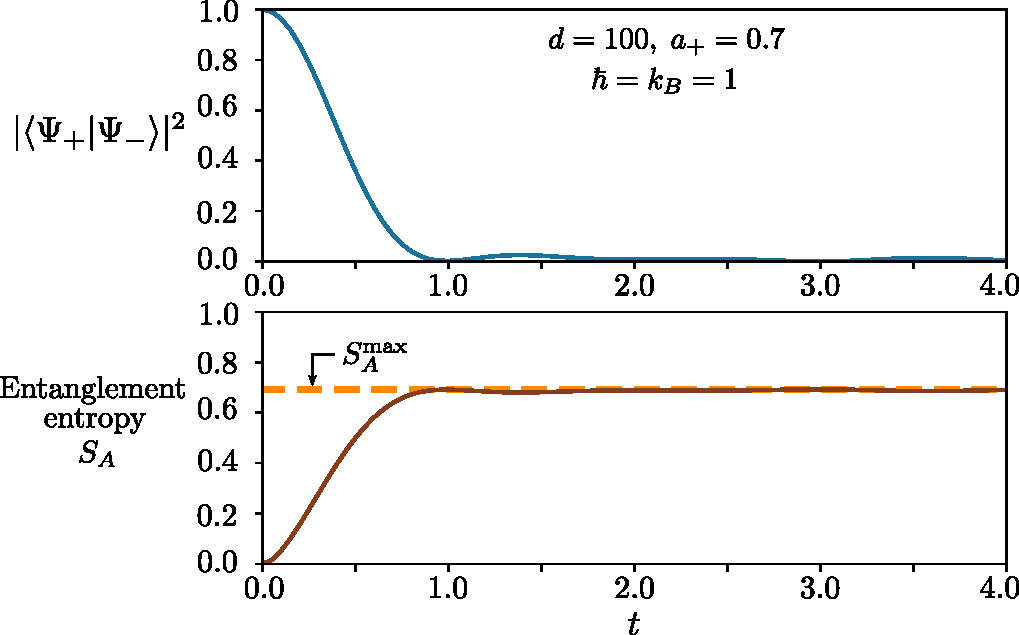
\includegraphics[width=0.7\textwidth]{decoherence}
\end{figure}

In the inital state, we let $a_+ = 0.7$, so $a_- = \sqrt{1-0.7^2} =
0.71414\dots$ The upper panel plots the overlap between the two
apparatus states, $|\langle\Psi_+|\Psi_-\rangle|^2$, versus $t$.  In
accordance with the preceding discussion, the overlap is unity at $t =
0$, but subsequently decreases to nearly zero.  For comparison, the
lower panel plots the entanglement entropy between the two subsystems,
$S_A = -k_b \mathrm{Tr}_A\left\{\hat{\rho}_A\ln\hat{\rho}_A\right\}$,
where $\hat{\rho}_A$ is the reduced density matrix obtained by tracing
over the spin subspace.  We find that $S_A = 0$ at $t=0$, due to the
fact that the spin and apparatus subsystems start out with definite
quantum states in $|\psi(0)\rangle$.  As the system evolves, the
subsystems become increasingly entangled, and $S_A$ increases up to
\begin{equation}
  S_A^{\mathrm{max}}/k_b = - \Big( |a_+|^2 \ln|a_+|^2 + |a_-|^2\ln|a_-|^2 \Big) \approx 0.693
\end{equation}
This value is indicated in the figure by a horizontal dashed line, and
corresponds to the result of the classical entropy formula for
probabilities $\{|a_+|^2,|a_-|^2\}$.  Moreover, we see that the
entropy reaches $S_A^{\mathrm{max}}$ at around the same time that
$|\langle\Psi_+|\Psi_-\rangle|^2$ reaches zero.  This demonstrates the
close relationship between ``measurement'' and ``entanglement''.

For details about the numerical linear algebra methods used to perform
the above calculation, refer to Appendix D.

The ``many worlds'' concept can be generalized from the above toy
model to the universe as a whole.  In the viewpoint of the Many Worlds
Interpretation of quantum mechanics, the entire universe can be
described by a mind-bogglingly complicated quantum state, evolving
deterministically according to the Schr\"odinger equation.  This
evolution involves repeated ``branchings'' of the universal quantum
state, which continuously produces more and more worlds.  The
classical world that we appear to inhabit is just one of a vast
multitude.  It is up to you to decide whether this conception of
reality seems reasonable.  It is essentially a matter of preference,
because the Copenhangen Interpretation and the Many Worlds
Interpretation have identical physical consequences, which is why they
are referred to as different ``interpretations'' of quantum mechanics,
rather than different theories.




\section*{Exercises}

\begin{enumerate}
%% \item A vector space $\mathscr{H}$ is said to have an inner product if
%%   there is an pairwise operation between its vectors that satisfies
%%   the following ``inner product axioms''.  For arbitrary
%%   $|\psi\rangle, |\psi'\rangle, |\psi''\rangle \in \mathscr{H}_A$,
%%   \begin{enumerate}
%%   \item $\langle \psi|\psi' \rangle = \langle\psi'|\psi\rangle^*$
%%   \item $\langle \psi|\psi \rangle \in \mathbb{R}^+_0$, and $\langle \psi|\psi \rangle = 0$ if and only if $|\psi\rangle = 0$.
%%   \item $\langle\psi| \, \big(|\psi'\rangle + |\psi'' \rangle\big)
%%     = \langle \psi|\psi'\rangle + \langle \psi|\psi''\rangle$
%%   \item $\langle \psi | \,\big(c|\psi'\rangle\big) = c\langle\psi|\psi'\rangle$ for all $c\in\mathbb{C}$,
%%   \end{enumerate}
%%   Prove that the inner product for $\mathscr{H}_A\otimes\mathscr{H}_B$
%%   defined in Section~\ref{sec:tensorprod} satisfies these axioms.
%%   \label{ex:innerprod}

\item Consider the density operator
  \begin{equation}
    \hat{\rho} = \frac{1}{2} |\!+\!z\rangle \langle+z|
    \,+\, \frac{1}{2} |\!+\!x\rangle \langle+x|
  \end{equation}
  where $|\!+\!x\rangle = \frac{1}{\sqrt{2}} \left(|\!+\!z\rangle +
  |\!-\!z\rangle\right)$.  This can be viewed as an equal-probability
  sum of two different pure states.  However, the density matrix can
  also be written as
  \begin{equation}
    \hat{\rho} \,=\, p_1\, |\psi_1\rangle \langle \psi_1|
    \,+\, p_2\, |\psi_2\rangle \langle\psi_2|
  \end{equation}
  where $|\psi_{1}\rangle$ and $|\psi_{2}\rangle$ are the eigenvectors
  of $\hat{\rho}$.  Show that $p_1$ and $p_2$ are \textit{not} 1/2.
  \label{ex:rho_decomp}


\item 
  Consider two distinguishable particles, $A$ and $B$.  The 2D Hilbert
  space of $A$ is spanned by $\{|m\rangle, |n\rangle\}$, and the
  3D Hilbert space of $B$ is spanned by $\{|p\rangle, |q\rangle,
  |r\rangle\}$.  The two-particle state is
\begin{equation}
  |\psi\rangle = \frac{1}{3} \, |m\rangle|p\rangle
+ \frac{1}{\sqrt{6}} \, |m\rangle|q\rangle
+ \frac{1}{\sqrt{18}} \, |m\rangle|r\rangle
+ \frac{\sqrt{2}}{3} \, |n\rangle|p\rangle
+ \frac{1}{\sqrt{3}} \, |n\rangle|q\rangle
+ \frac{1}{3} \, |n\rangle|r\rangle.
\end{equation}
Find the entanglement entropy.

\end{enumerate}

\section*{Further Reading}

\begin{enumerate}[[1{]}]
\item Bransden \& Joachain, \S14.1---14.4, \S17.1--17.5

\item Sakurai, \S3.9

\item A.~Einstein, B.~Podolsky, and N.~Rosen,
  \textit{Can Quantum-Mechanical Description of Physical Reality Be
    Considered Complete?}, Physical Review \textbf{47}, 777 (1935).
  [\href{https://journals.aps.org/pr/abstract/10.1103/PhysRev.47.777}{link}]
  \label{cite:epr}

\item J.~S.~Bell, \textit{On the Einstein-Podolsky-Rosen paradox},
  Physics \textbf{1}, 195 (1964). [\href{http://inspirehep.net/record/31657/files/}{link}]\label{cite:bell}
  
\item N.~D.~Mermin, \textit{Bringing home the atomic world: Quantum
  mysteries for anybody}, American Journal of Physics \textbf{49}, 940
  (1981). [\href{http://aapt.scitation.org/doi/abs/10.1119/1.12594}{link}] \label{cite:mermin}

\item A.~Aspect, \textit{Bell's inequality test: more ideal than ever},
  Nature (News and Views) \textbf{398}, 189 (1999). [\href{https://www.nature.com/articles/18296}{link}] \label{cite:aspect}

\item A.~K.~Ekert, \textit{Quantum Cryptography Based on Bell's Theorem},
  Physical Review Letters \textbf{67}, 661 (1991). [\href{https://journals.aps.org/prl/abstract/10.1103/PhysRevLett.67.661}{link}] \label{cite:ekert}

  
\item H.~Everett, III, \textit{The Theory of the Universal Wave
  Function} (PhD thesis), Princeton University (1956)
  [\href{http://ucispace.lib.uci.edu/handle/10575/1302}{link}]
\label{cite:everett}

\item A.~Albrecht, \textit{Following a ``collapsing'' wave function},
  Physical Review D \textrm{48}, 3768 (1993). [\href{https://journals.aps.org/prd/abstract/10.1103/PhysRevD.48.3768}{link}]
\label{cite:albrecht}

\item A.~Edelman and N.~R.~Rao, \textit{Random matrix theory}, Acta
  Numerica \textbf{14}, 233 (2005). [\href{https://doi.org/10.1017/S0962492904000236}{link}]
\label{cite:edelman}
\end{enumerate}

\end{document}


%% For decades after the discovery of quantum mechanics, the quantum
%% double-slit experiment was just a ``thought experiment'', meant to
%% illustrate the features of quantum mechanics that had been uncovered
%% by other, more complicated experiments.  Nowadays, the most convenient
%% way to do the experiment is with light, using single-photon sources
%% and single-photon detectors.  Quantum interference has also been
%% demonstrated experimentally using electrons, neutrons, and even
%% large-scale particles such as buckyballs.
